\documentclass[11pt]{beamer}
\usetheme{Goettingen}
\usepackage[utf8]{inputenc}
\usepackage{amsmath}
\usepackage{amsfonts}
\usepackage{amssymb}
\usepackage{graphicx}
\usepackage{hyperref}
\author{Alex Heilman}
\title{Point Group Equivariant Networks for Material Systems}
\subtitle{Thesis Proposal}
%\setbeamercovered{transparent} 
%\setbeamertemplate{navigation symbols}{} 
%\logo{} 
%\institute{} 
%\date{} 
%\subject{} 


\addtobeamertemplate{navigation symbols}{}{%
	\usebeamerfont{footline}%
	\usebeamercolor[fg]{footline}%
	\hspace{1em}%
	\insertframenumber/\inserttotalframenumber
}


%Global Background must be put in preamble


\usepackage[style=numeric,backend=bibtex,sorting=none]{biblatex}

\addbibresource{chgcnn.bib}
\addbibresource{chgcnn.bib}


\newenvironment{boxed2}
    {\begin{center}
    \begin{tabular}{|p{0.95\textwidth}|}
    \hline\\
    }
    { 
    \\\\\hline
    \end{tabular} 
    \end{center}
    }


\begin{document}

\begin{frame}
\titlepage
\end{frame}

\begin{frame}{Overview}
	Graph Neural Networks for Materials Science
	
	\vspace{0.5cm}
	
	$\bullet$ Hypergraph representations
	
	\vspace{0.5cm}
	
	$\bullet$ Importance of Equivariance
	
	\vspace{0.5cm}
	
	$\bullet$ $O(3)$ Equivariance \& Tensor Predictions
	
	\vspace{0.5cm}
	
	$\bullet$ Why we should use material symmetry groups!
\end{frame}

%\begin{frame}
%\tableofcontents
%\end{frame}


\begin{frame}{Why Neural Networks?}
	Physics assumes there exists a map between configurations and properties of physical systems: 
	$$
	\lbrace\vec{r}_i \rbrace \xrightarrow[\text{Nature}]{}
	\lbrace\vec{r}_i' \rbrace
	$$
	Neural network techniques assume maps between abstract input and output spaces exist:
	$$
	X
	\xrightarrow[\text{Neural Network}]{}
	Y
	$$
	These may be expressed in a basis of adequately large neural networks \cite{universal1}.
	
	\vspace{0.5cm}
	
	\begin{center}
		But how do we apply this to material systems?
	\end{center}
	
\end{frame}

\begin{frame}{Machine Learning on Crystal Systems}
To perform predictive tasks for material systems, we need two things:

\vspace{0.6cm}

$1.$ A way to represent the system mathematically

\vspace{0.3cm}

$2.$ A trainable model that acts on this representation
\end{frame}


\section{Graph Neural Networks}
\begin{frame}{Usual Crystal Graph Construction \small(a la CGCNN)}

$\bullet$ Common techniques represent crystalline systems as graphs (nodes and edges) \cite{cgcnn, schnet, megnet}

\vspace{.3cm}

$\bullet$ Associate atomic features with nodes and geometric features with edges

\vspace{.6cm}

\begin{center}

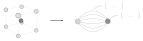
\includegraphics[scale=0.7]{crystalgraph.pdf}

\vspace{.3cm}

How do we construct these?

\end{center}

\end{frame}

\begin{frame}{Crystal Graphs cont. I}

$\bullet$ Edges are determined by distance cutoff (8 Ang.) and maximum number of neighbors (12)

\begin{center}
\includegraphics[scale=0.45]{ex_bondcriteria.pdf}
\end{center}
\end{frame}

\begin{frame}{Crystal Graphs cont. II}
$\bullet$ Edge attributes $e$ then are a Gaussian distance expansion

\begin{center}
\includegraphics[scale=0.33]{bond_feat.pdf}
\end{center}
\end{frame}

\begin{frame}{Crystal Graphs cont. III}
	
	\vspace{1cm}
	
	$\bullet$ Node features $n$ are encoded physical properties
	\begin{center}
		\includegraphics[scale=0.33]{atom_feat.pdf}
		
		\vspace{1cm}
		
	What do we do with these things?
	\end{center}
\end{frame}

\begin{frame}{Message Passing on Graphs}
Update with GNN or message passing network \cite{mpnn}:
\begin{gather*}
m_i^{t+1}=\sum_{n_j\in \mathcal{N}(i)} M_t(n_i^{t},e_{ij},n_j^t )\\
\\
n_i^{t+1}=U_t(n_i^t,m_i^{t+1})\\
\end{gather*}
%Here, each node $n$ from layer $t$ to $t+1$ is updated according to an update function $U$, which takes as input messages formed from each pair of nodes containing the node to be updated.
Then, read out prediction from updated node features.
\end{frame}

\begin{frame}{Continuous Filters}
Atomic interactions are very sensitive to distance!

\vspace{0.2cm}

$\bullet$ Continuous-resolution convolutional filters \cite{schnet}

\vspace{0.2cm}

$\bullet$ CGConv \cite{cgcnn}:

\begin{align*}
	n_i^{t+1} &= \sum_{b_j} f(n_i^t, b_j,\text{AGG}(\lbrace n_j^t\in b_j \rbrace )) \\ 
	& = \text{BN}\bigg[\sum_{b_j}\sigma \big(W_c\cdot [n_j\oplus e_{ij}\oplus n_j\big)\\
	&\quad\quad\quad\quad\cdot S^+ (W_f\cdot (n_j\oplus  e_{ij}\oplus n_j ) \bigg]
\end{align*}
\end{frame}

\begin{frame}{Graph Neural Network}
	
	\vspace{-0.5cm}
	
\begin{center}
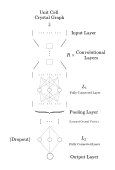
\includegraphics[scale=0.53]{cgcnnarch.pdf}
\end{center}
\end{frame}

\begin{frame}{Graph Limitations}
Problem: Our underlying representation encodes only distances between atoms!

\begin{center}

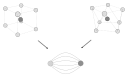
\includegraphics[scale=0.7]{crystalgraph_cntex.pdf}

\medskip

These two have the same representations!
\end{center}
\end{frame} 

\subsection{Crystal Hypergraphs}
\begin{frame}{(One) Solution: Hypergraphs!}
Hypergraphs allow us to have edges containing more than (or less than) two nodes.

\begin{center}
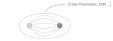
\includegraphics[scale=0.6]{motiflevel_ex.pdf}
\end{center}

$\bullet$ Gives a natural way to encode features with higher order structure

\vspace{.3cm}

$\bullet$ Hypergraph nodes still represent atoms of underlying crystal structure.

\vspace{.3cm}

$\bullet$ Treat all different order structures on equal footing: each has a corresponding hyperedge with a feature

\vspace{.15cm}

\begin{center}
	But what do we care about?
\end{center}
\end{frame}


\begin{frame}{Coordination Environments as Hyperedges}


Considering the previous problem; encode coordination environment in larger hyperedges.

\medskip

\begin{center}

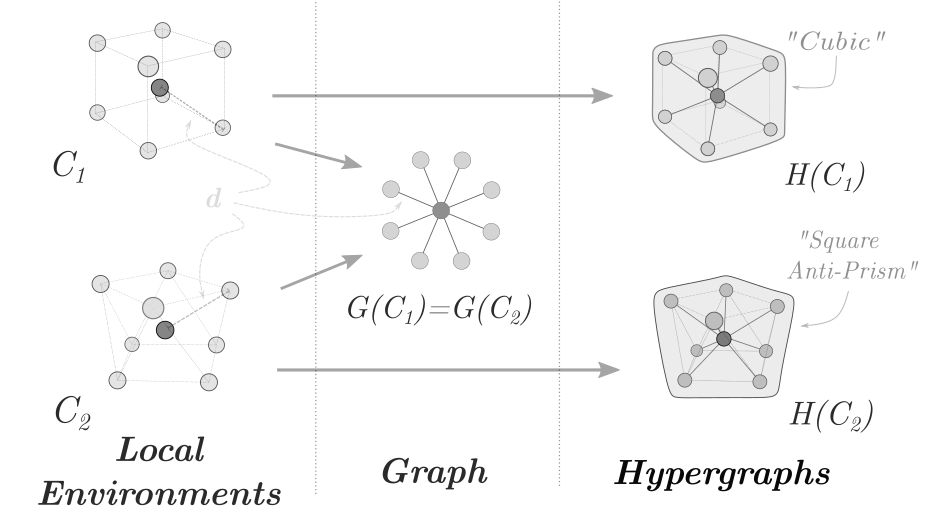
\includegraphics[scale=0.34]{../chgcnn/chgcnn_revised_3/graph2hgraph_tall_revise2.pdf}

\end{center}

\medskip

$\bullet$ Geometrical information can be encoded quantitatively with continuous symmetry measures, local structure order parameters, etc.


\end{frame}


\begin{frame}{Extending Message Passing to Hypergraphs}

Now, we need a suitable convolutional structure that applies to hypergraphs...



\begin{gather*}
m_i^{t+1}=\sum_{h_j\ni x_i} M_t(n_i^{t},\underbrace{h_j^{t},\lbrace  n_w^t \vert n_w \in h_j }_{e_{ij},n_j}\rbrace)\\
\\
n_i^{t+1}=U_t(n_i^t,m_i^{t+1})\\
\end{gather*}

\medskip

$\bullet$ Neighborhoods of nodes relevant to each message are now a set

\begin{center}
What can we do?
\end{center}

\end{frame}



\begin{frame}{Hypergraph Convolution}
\begin{center}
Aggregate the node features!
\end{center}
\begin{align*}
n_i \rightarrow n_i &+ \sum_{e_{ij}}M_b(n_i\oplus e_{ij} \oplus n_j)\\
&+ \sum_{h_j}M_m(n_i\oplus h_{j} \oplus \text{AGG}(\lbrace  n_w^t \vert n_w \in h_j \rbrace))
\end{align*}

$\bullet$ AGG can be maximum, minimum, mean, standard deviation

\vspace{0.3cm}

$\bullet$ Can also be learnable mix of above with attention

\end{frame}

\begin{frame}{CHGConv}
A generalization of CGConv with hyperedge aggregation:

\begin{align*}
	n_i^{t+1} &= n_i^t + \sum_{b_j} f(n_i^t, b_j,\text{AGG}(\lbrace n_j^t\in b_j \rbrace )) \\ 
	& =  n_i^t + \text{BN}\bigg[\sum_{b_j}\sigma \big(W_c\cdot [n_j\oplus b_j\oplus \text{AGG}(\lbrace n_j^t\in b_j \rbrace ] )\big)\\
	&\quad\quad\quad\quad\quad\quad\cdot S^+ (W_f\cdot (n_j\oplus b_j\oplus \text{AGG}(\lbrace n_j^t\in b_j \rbrace ) )  ) \bigg]
\end{align*}
\end{frame}

\begin{frame}{CHGCNN Schematic}
\begin{center}
	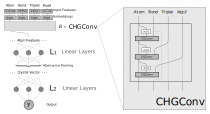
\includegraphics[scale=0.45]{arch_horiz.pdf}
\end{center}

\vspace{0.3cm}

\end{frame}

\begin{frame}{CHGCNN Results}
	
\hspace{-0.1cm}{\footnotesize
\begin{tabular}{|c|c|c|c|}
\hline
Hyperedge & $E_g$  & $G_{vrh}$ & $K_{vrh}$ \\
Types & MAE (eV)   & MAE (Log$_{10}$GPa)& MAE (Log$_{10}$GPa)    \\
\hline
Bond-Only    & 0.257  & 0.0826 & 0.0688 \\
 Bond \& Motif & 0.232  &0.0813&0.0623  \\
\hline
\end{tabular}}


\vspace{0.7cm}

$\bullet$ Allows us to effectively capture higher-order geometric features, in an \textit{invariant} manner!

\vspace{0.35cm}

\begin{center}
	But what if we care about about coordinate-system dependent quantities?
\end{center}

\end{frame}

\section{$O(3)$-Equivariant Networks}

\begin{frame}{Equivariant Functions}
	A function $f:X\rightarrow Y$ is \textit{equivariant} if it 'commutes' with a group:
	$$
	f\Big(\mathcal{D}^X(g)x\Big)=\mathcal{D}^Y(g)f(x)
	$$
	
	\vspace{0.35cm}

	$\bullet$  $X,Y$ are vector spaces

	\vspace{0.2cm}

	$\bullet$ $\mathcal{D}$ are group representations of elements $g$

	\vspace{.6cm}
	
	Note: Equivariance is always with respect to some group!
\end{frame}
\begin{frame}{Why Equivariant Functions?}
	\begin{center}
		Physical processes respect coordinate system rotations $R$:
		$$
		\lbrace R\vec{r}_i \rbrace \xrightarrow[\text{Nature}]{}
		\lbrace R\vec{r}_i' \rbrace
		$$
		
		\vspace{0.6cm}
		
		In general, neural networks do not:
		$$
		RX
		\xrightarrow[\text{Neural Network}]{} \ \ 
		?
		$$
		
		So what do we want?
		
	\end{center}
\end{frame}
\begin{frame}{Equivariant Networks}
	\begin{center}
		We want equivariant networks for physics!
		
		$$
		RX
		\xrightarrow[\text{Neural Network}]{\text{Equivariant}} RY
		$$
		
		\vspace{0.6cm}
		
	\end{center}
	
	In equivariant networks, we consider feature vectors in basis of representation space:
	$$
	v^{\alpha}_i
	$$
	Index $\alpha$ denotes irrep, and $i$ the dimension of irrep space $\alpha$.
	
	
\end{frame}
\begin{frame}{Equivariant Networks (cont.)}
	Compositions of equivariant functions are equivariant \cite{equivariant_cohen}. We consider building blocks:{\small
		\begin{itemize}
			
			\item Self-interaction:
			$$
			v'_{nc} = W^{c'}_c v_{nc'}
			$$
			\item Non-linear functions along channels  (for trivial irrep $\alpha=1$):
			$$
			v'_{nc}=f(v_{nc}+b_{nc})
			$$
			\item Group correlation with filters \cite{equivariant_cohen}:
			$$
			[F\star v](g)=\sum_{h\in G}\sum_c F_c(h)v_c(g^{-1}h)
			$$
			\item Tensor products with filters \cite{tensorfieldnetworks, e3nn}:
			$$
			(v'_{nc})^{\gamma}_{n} = \sum_{ij}U_{\alpha i \beta j}^{\gamma n}\big(F_{j}^{\beta}\otimes V^{\alpha}_i \big) 
			$$
			\item Pooling over nodes or channels:
			$$
			v_c = \sum_n v_{nc}
			$$
	\end{itemize}}
\end{frame}
\begin{frame}{$SO(3)$ Properties}
	Most modern equivariant networks are specifically $SO(3)$-Equivariant.
	
	\vspace{0.5cm}
	
	\begin{itemize}
		\item Inifinite order $\rightarrow$ infinite irreps
		\item Irreps are Wigner $\mathcal{D}^{\ell}$ matrices
		\item Natural basis set $Y^{\ell}_m$ of dimension $d_{\ell}=2\ell+1$
	\end{itemize}
	
	\vspace{0.5cm}
	
	Many models are further referred to as $E(3)$-equivariant \cite{e3nn} for the Euclidean group (add parity and translation invariance).
\end{frame}

\begin{frame}{\textit{Tensor Field Networks}}
	Tensor field networks \cite{tfn} use SO(3) equivariant convolution:{\small
		$$
		\big(v^{L+1}_{nc}\big) ^{\ell}_{m}=\big(v^{L}_{nc}\big)^{\ell}_m+\sum_{b\in \mathcal{N}(n)}\sum_{\ell_f m_f , \ell_i m_i}^{\ell_{\text{max}} m_{\text{max}}}c_{\ell_fm_f\ell_im_i}^{\ell m}\big(F^{L}_c(r_{nb})\big)^{\ell_f}_{m_f}\big(v_{bc}^L \big)^{\ell_i}_{m_i}
		$$}
	\begin{itemize}
		\item $v_{nc}^{L}$: Node feature of node $n$, channel $c$, layer $L$
		\item $c_{\ell_fm_f\ell_im_i}^{\ell_om_o}$: Clebsch-Gordan coefficients
		\item $F_c^L$: Filter function (trainable)
		\item $r_{nb}$: Radius between nodes $n$ and neighbor $b\in \mathcal{N}(n)$
	\end{itemize}
	
	\vspace{.7cm}
	
	$F$ is generally a neural network; $r$ is often expanded with some radial basis function (RBF): Gaussian, Bessel, etc.
\end{frame}

\begin{frame}{$SO(3)$-Equivariant Features}
	Remember that node (and edge) features now have additional indices $\ell$ and $m$!
	$$
	\big(v^{L+1}_{nc}\big) ^{\ell}_{m}
	$$	
	
	This allows us to keep track of which components transform like which irreps of $SO(3)$.
	
	\vspace{0.6cm}
	
	\begin{center}
	But what can we do with this?
	\end{center}
\end{frame}

\subsection{Tensor Prediction}


\begin{frame}{$J_z$ Basis}
	Recall $\ell=1$ spherical harmonics (with Racah normalization):
	\begin{align*}
		Y_1^{+1} &= -\frac{1}{\sqrt{2}}(x+iy)=\frac{1}{\sqrt{2}}\sin \phi e^{i\theta}\\
		Y_1^{0}\ \ &= z = \cos \phi\\
		Y_1^{-1} &= -\frac{1}{\sqrt{2}}(x-iy)=\frac{1}{\sqrt{2}}\sin \phi e^{-i\theta}
	\end{align*}
	\begin{center}
		Define $J_z$ basis \cite{mochizuki1988spherical,mochizuki1996spherical}:
		$$
		\begin{bmatrix}
			a_+ \\
			a_0 \\
			a_-
		\end{bmatrix}=\begin{bmatrix}
			-\frac{1}{\sqrt{2}} & -\frac{i}{\sqrt{2}} & 0\\
			0 & 0 & 1\\
			-\frac{1}{\sqrt{2}} & +\frac{i}{\sqrt{2}} & 0\\
		\end{bmatrix}\begin{bmatrix}
			x \\
			y \\
			z
		\end{bmatrix}
		$$
		so that $\vec{n}=a_+ \hat{Y}_1^1 + a_0 \hat{Y}_1^0 + a_- \hat{Y}_1^{-1}$
	\end{center}
\end{frame}
\begin{frame}{Clebsch-Gordon Expansion}
	Build larger spherical harmonic tensors with CG expansion:
	$$
	Y_{\ell_1}^{m_1}\otimes Y_{\ell_2}^{m_2} = \sum_{L=|\ell_1-\ell_2|}^{\ell_1+\ell_2}\sum_{M=-L}^{L}c_{\ell_1 0 \ell_2 0}^{L0}c_{\ell_1 m_1 \ell_2 m_2}^{LM}Y_{L}^M
	$$
	\cite{sakurai} where $Y_{L}$ represents a $2L+1$ dimensional symmetric tensor space of rank $L$. 
	
	\vspace{0.5cm}
	
	$\bullet$ Gives a relation between symmetric tensor's $J_z$ basis components and other spherical harmonic tensors. 
	
	$$ 
	T^{(n)} = a_{\underbrace{\alpha\beta...}_n}\big(Y_1^\alpha \otimes Y_1^\beta\otimes ... \big)\ \  \Rightarrow\ \  y_\ell^m Y_L^M
	$$
	
	\begin{center}
		But, what about asymmetric tensors?
	\end{center}
\end{frame}
\begin{frame}{$SO(3)$ Invariant Tensor Subspaces}
	$\bullet$ An arbitrary tensor $T$ transforms as:
	$$
	T_{x_1x_2...x_n}\rightarrow T_{x'_1x'_2...x_n'}=R_{x_1'}^{x_1} R_{x_2'}^{x_2} R_{x_3'}^{x_3}T_{x_1x_2...x_n},
	$$
	
	\vspace{0.5cm}
	
	$\bullet$ $T$ may be broken into a set of irreducible (but not necessarily unique) symmetric, $SO(3)$ invariant subtensors:
	$$
	\lbrace h^{(\ell)}\rbrace \rightarrow \lbrace h'^{(\ell)}\rbrace = \lbrace \mathcal{D}^{\ell}(R) h^{(\ell)}\rbrace
	$$
	
	\vspace{0.5cm}
	
	$\bullet$ This decomposition can be constructed by consecutive decomposition with respect to $GL$ and then $O$ and $SL$
	$$
	SO= (SL\cap O) \subset GL
	$$
\end{frame}

\begin{frame}{Decomposition Example: Rank 2}
	\begin{center}
Consider a rank-two tensor $T_{ij}$:
$$
S_{ij}=\frac{1}{2}(T_{ij}+T_{ji})
$$
$$
A_{ij}=\frac{1}{2}(T_{ij}-T_{ji})
$$

	\vspace{0.4cm}

	Then, contract with $g$ and $\varepsilon$:
	
	\vspace{0.5cm}
	
	\includegraphics[scale=0.33]{rank2-ex.pdf}
	
	\vspace{1.5cm}
\end{center}
\end{frame}




\begin{frame}{Model Architecture}
\begin{center}
	\includegraphics[scale=0.35]{tensor_arch.pdf}
\end{center}
\end{frame}


\begin{frame}{Tensor Prediction: Examples}
	Applications to materials:
	
	\vspace{0.3cm}
	
	$\bullet$ Dielectric Tensor $\epsilon_{ij}$
		
				\includegraphics[width=0.6\linewidth]{../spherical-elastic/segnn_default_dielectric_heatmap.pdf}
		
\end{frame}
	\begin{frame}{Tensor Prediction: Examples}
	$\bullet$ Piezoelectric Tensor $d_{ijk}$
	
			\includegraphics[width=0.8\linewidth]{../spherical-elastic/segnn_default_piezo_heatmap.pdf}
		
\end{frame}
\begin{frame}{Tensor Prediction: Examples}
	$\bullet$ Elasticity Tensor $C_{ijkl}$
		\includegraphics[width=0.9\linewidth]{../spherical-elastic/segnn_default_elastic_heatmap.pdf}
\end{frame}



\begin{frame}{Tensor Prediction with $SO(3)$-Networks}
	
	\begin{tabular}{|c|ccc|}
		\hline
		\textbf{Target}& \multicolumn{3}{|c|}{MAE (Averaged Over Components)} \\
		 \textbf{Components} & SEGNN & SEConv & SETransformer\\
		\hline 
		Elastic  \textit{[GPa]}& 8.139 & 7.689 & 7.941 \\
		Dielectric & 4.82 &4.702 &4.718\\
		Piezoelectric \textit{[C/$m^2$]} & 0.170 & 0.170 & 0.1714\\
		\hline
	\end{tabular}
	
	\vspace{0.8cm}
	
	$\bullet$ We can read off the output of $SO(3)$-networks as tensor components 
	
	\vspace{0.25cm}
	
	$\bullet$ These naturally respect coordinate transformations acting on the input space!
	
	\vspace{0.25cm}
	
	$\bullet$ Can learn, but doesn't restrict to symmetry of crystals...
	
	\vspace{0.4cm}
	
	\begin{center}
		Can we get more out of symmetry considerations?
	\end{center}
\end{frame}

\section{Material Symmetry}
{
	\usebackgroundtemplate{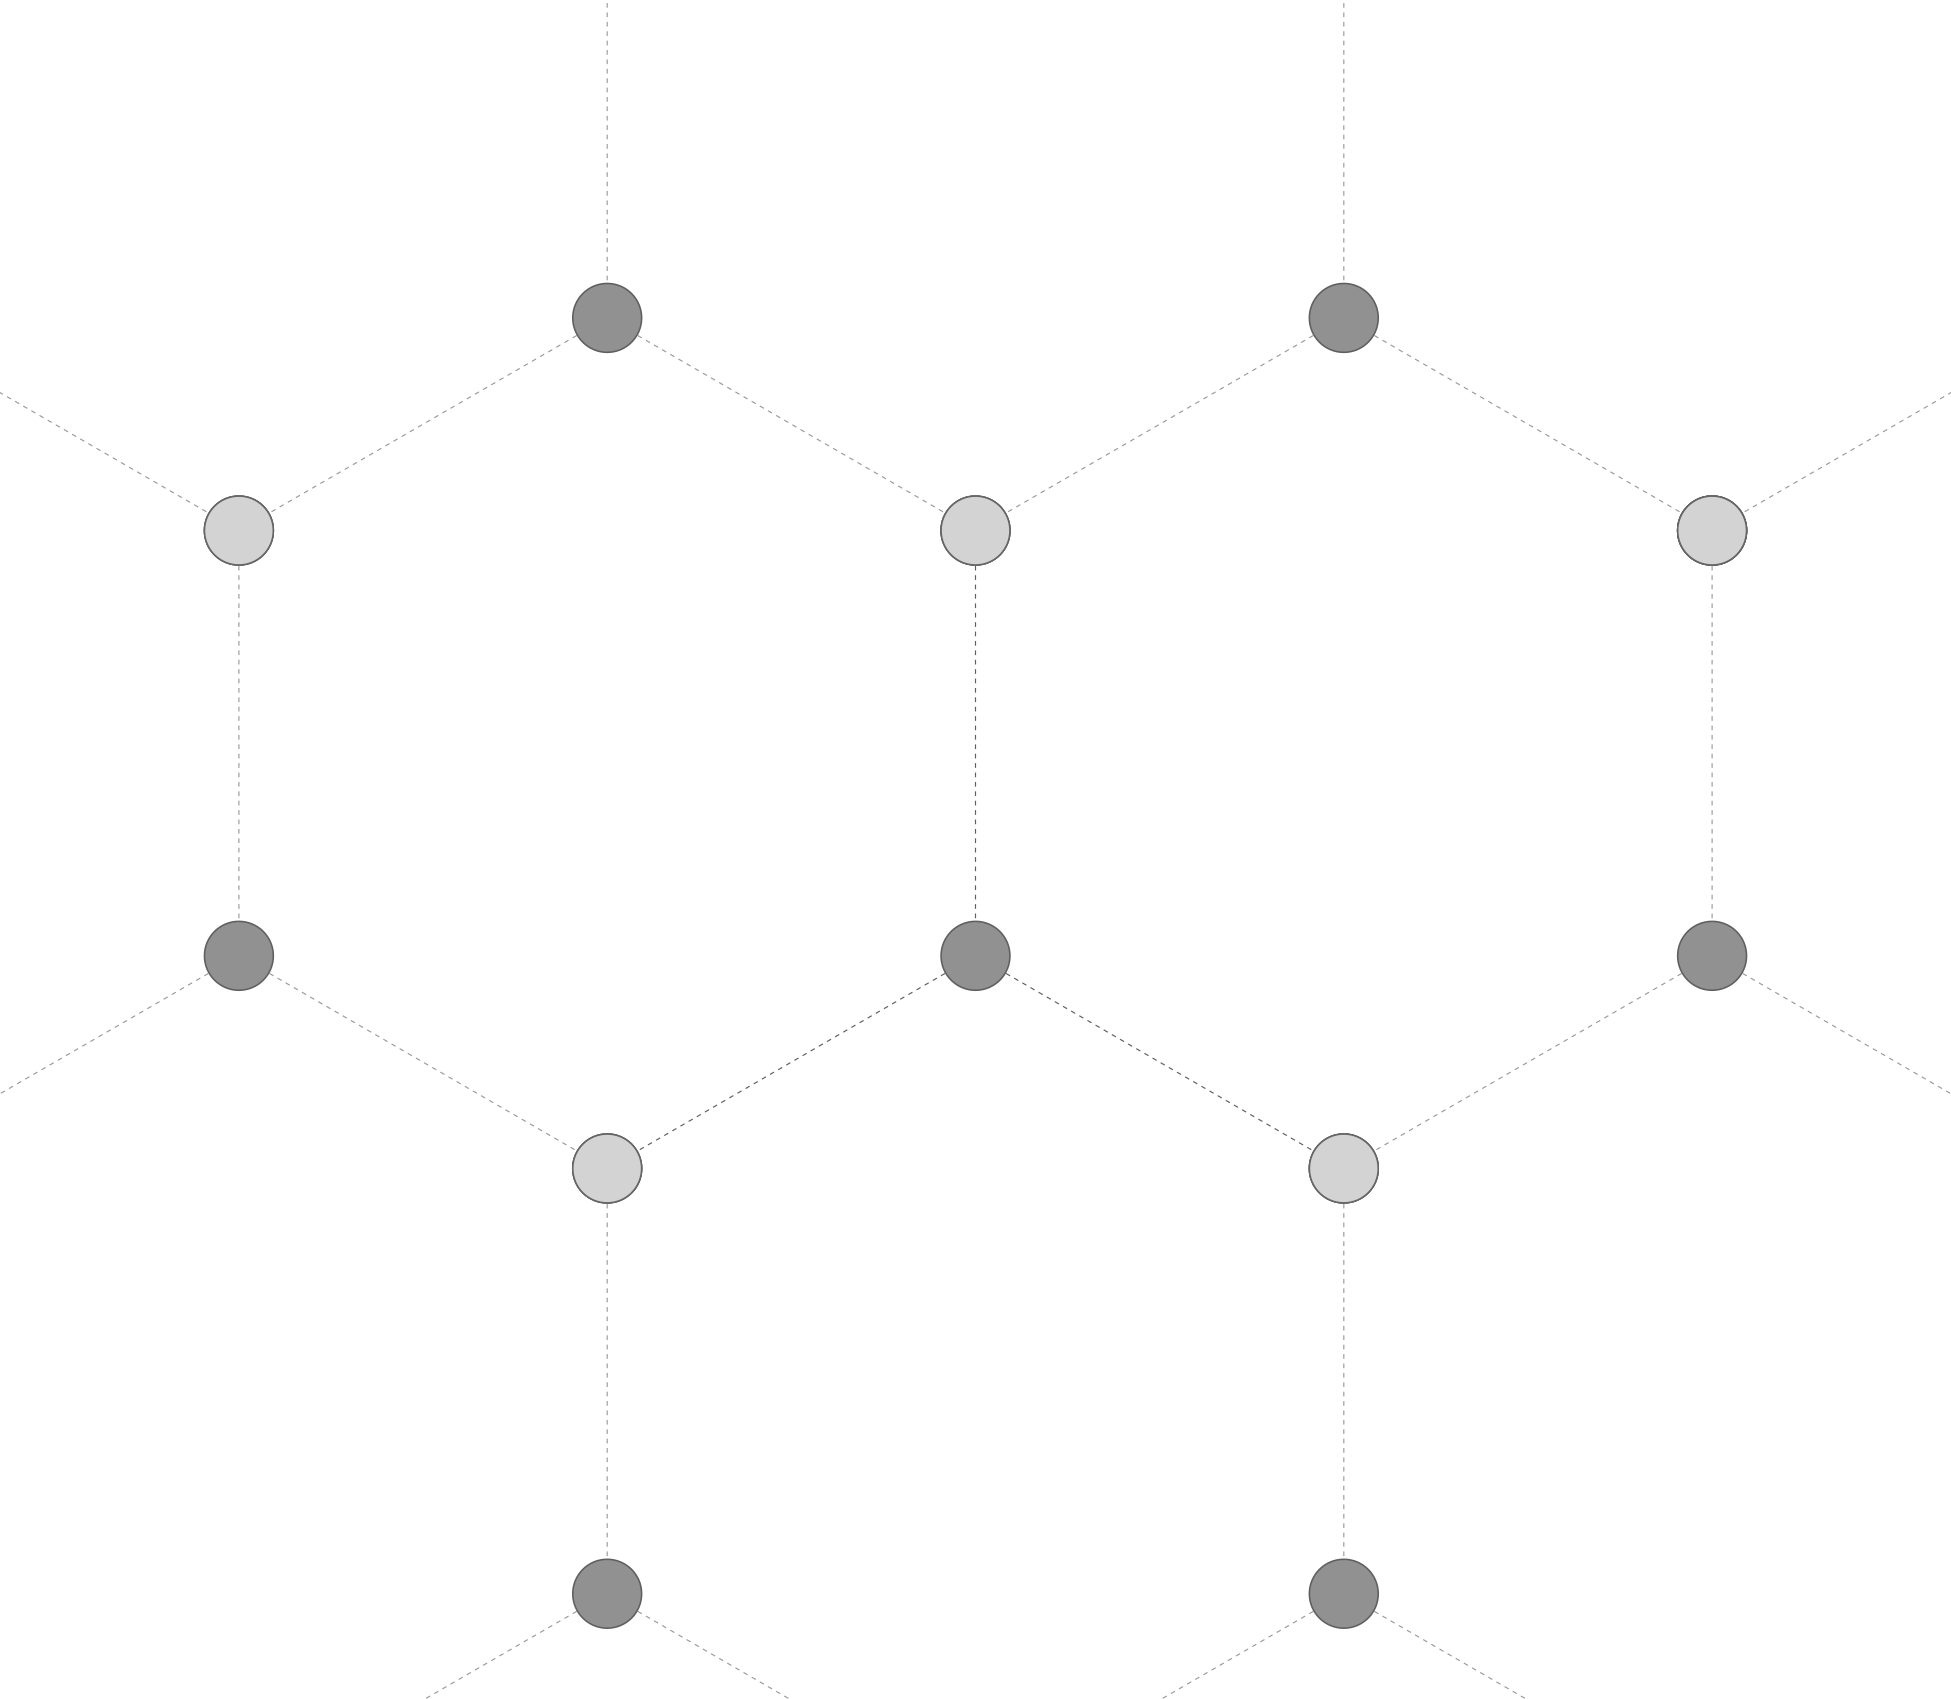
\includegraphics[width=\paperwidth]{pg_schem.pdf}}%
\begin{frame}{Material Symmetries}
\begin{center}
%	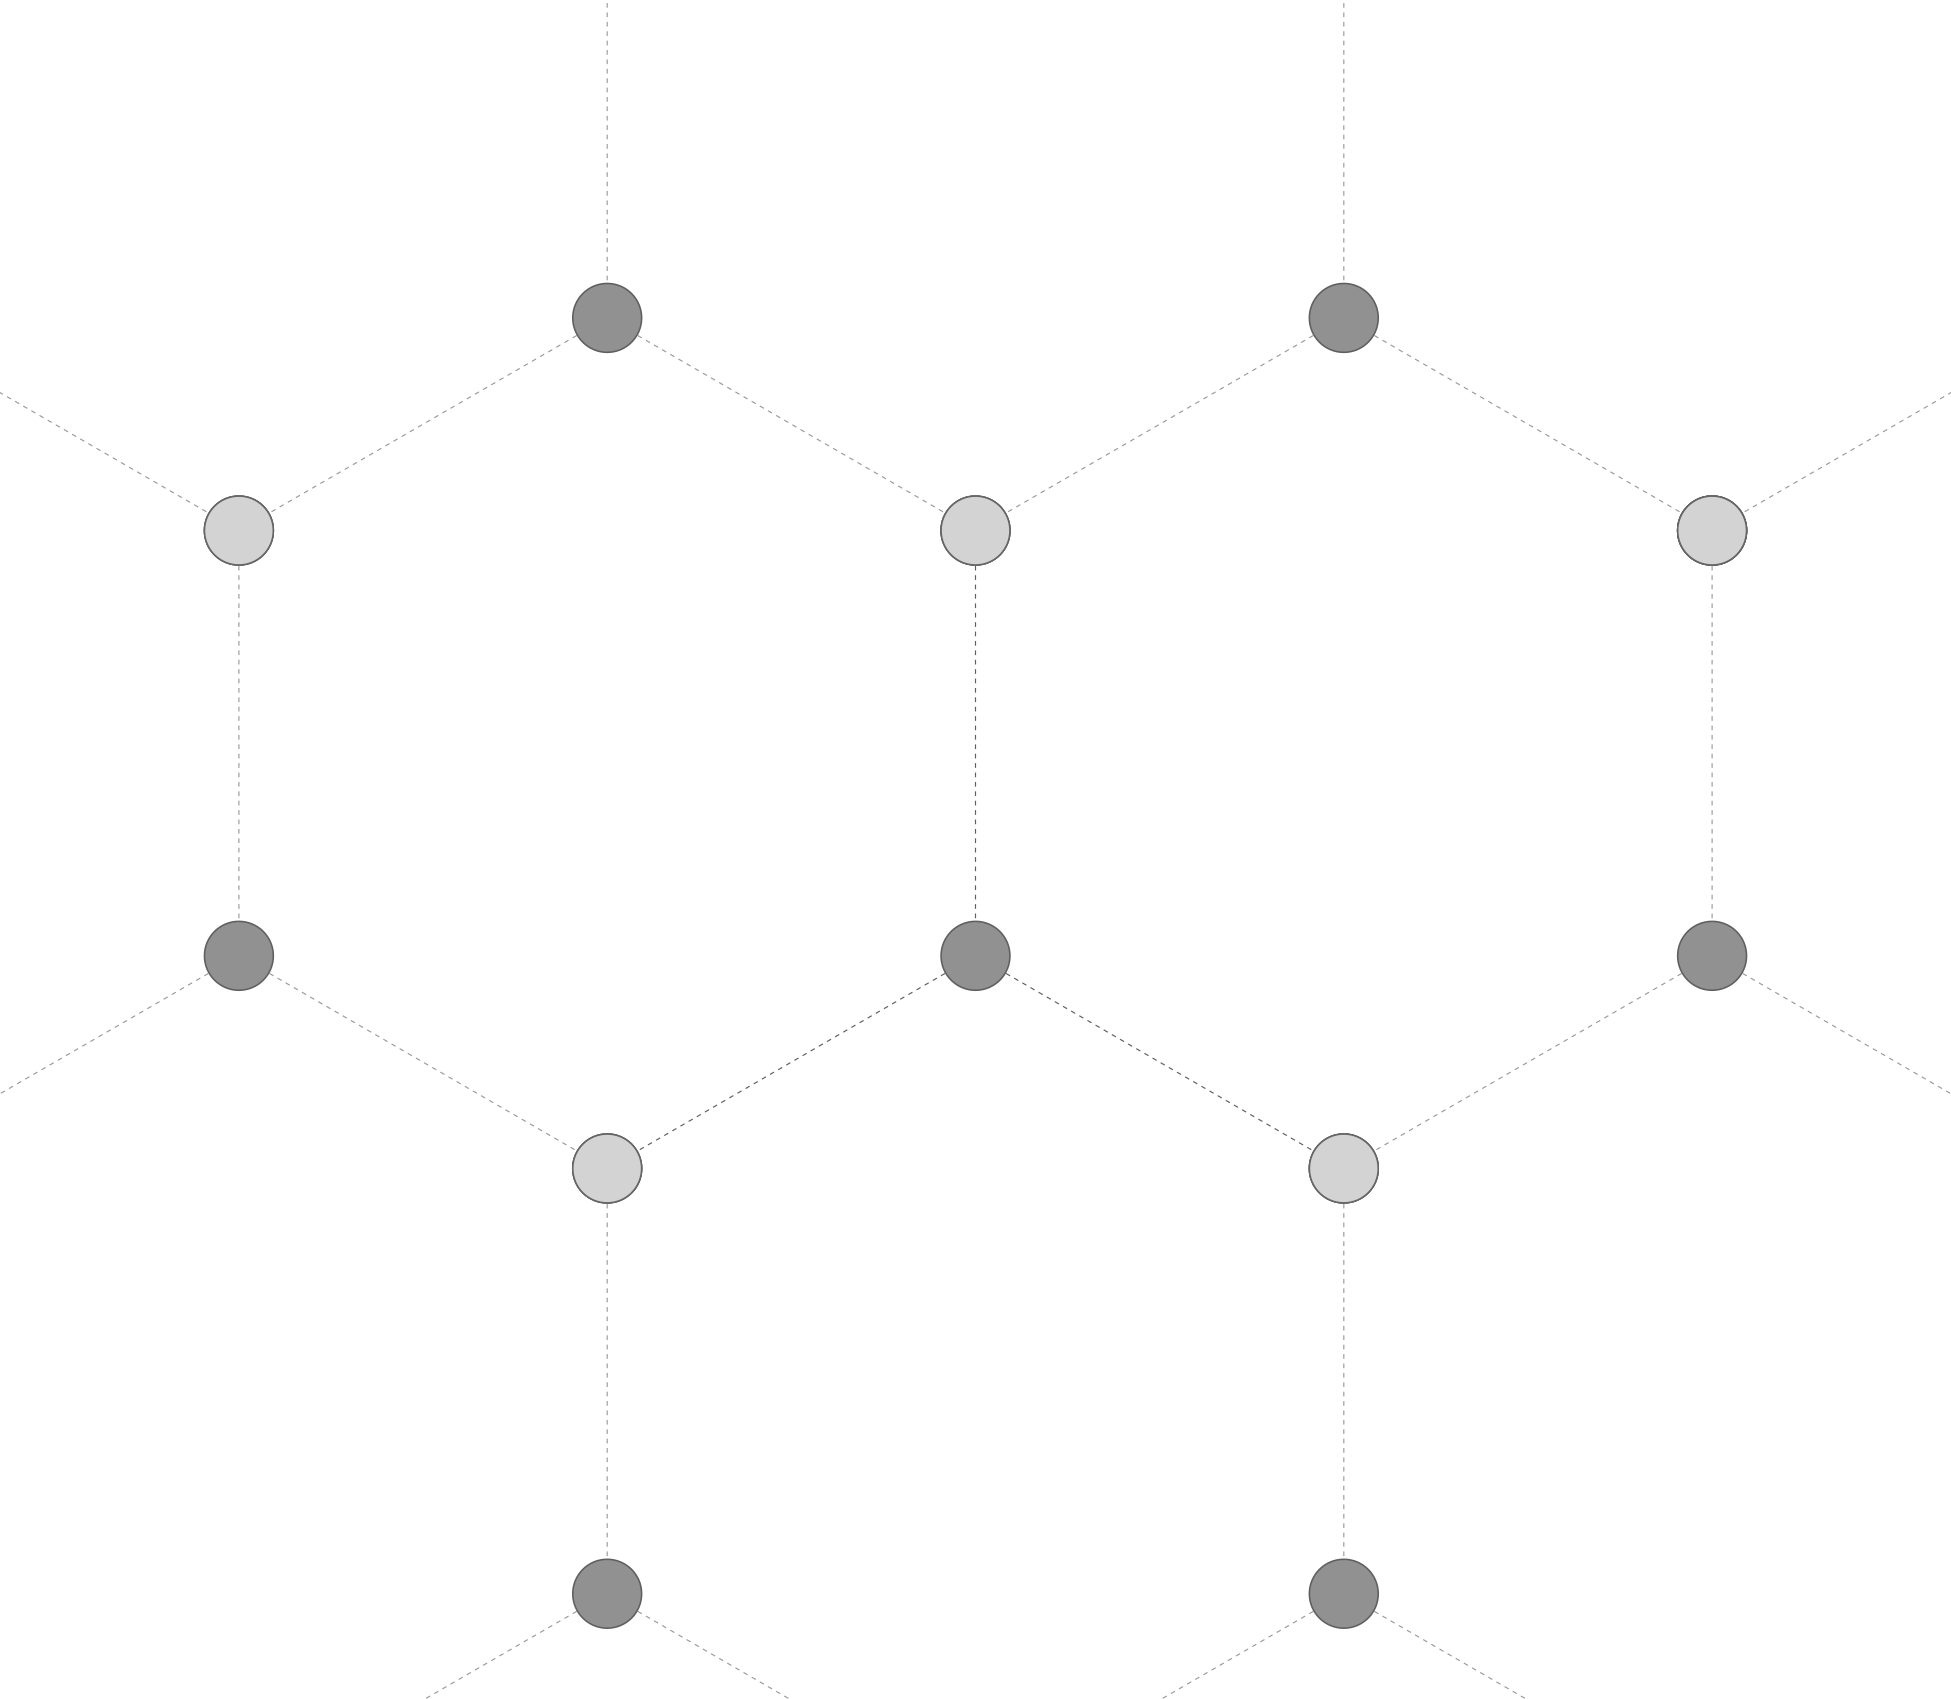
\includegraphics[scale=0.16]{pg_schem.pdf}
\end{center}
\end{frame}
}


\begin{frame}{Point Group Properties}
	Groups of operations that leave at least one point fixed and are compatible with a Bravais lattice.
	
	\vspace{0.3cm}
	
	Point groups (in 3D) have following properties:
	\begin{itemize}
		\item 32 crystallographic point groups in 3D
		\item Finite number of irreps for each
		\item All irreps of point groups are of dimension $d_{\alpha}=1,2,3$
		\item All allow a (often reducible) 3D representation
		\item Decompositions with $c_{\alpha\beta\gamma}=0,1,2$
	\end{itemize}
	
	{\small
		(Point group representations may be used to generate induced representations of space groups)}
\end{frame}

\begin{frame}{Site-symmetry Equivariant Networks}
	\begin{center}
		Index vectors by $\alpha ,i$  from site-symmetry group instead!
	\end{center}
	{\small
		$$
		\big(v^{L+1}_{nc}\big) ^{\gamma}_{n}=\big(v^{L}_{nc}\big)^{\gamma}_n+\sum_{b\in \mathcal{N}(n)}\sum_{\alpha i, \beta j}U_{\alpha i \beta j}^{\gamma n}\big(F^{L}_c(r_{nb})\big)^{\beta }_{j}\big(v_{bc}^L \big)^{\alpha}_{i}
		$$}
	
	\begin{itemize}
		\item Natural cutoff (finite summation over $\alpha,\beta$)
		\item Natural readout for symmetric properties ($\gamma=1$)
		\item Accounts for all physical symmetry but not more
	\end{itemize}
	
\end{frame}

\begin{frame}{Applications}

With these models, I propose  we can predict:

\vspace{0.4cm}

$\bullet$ Scalar quantities that are invariant under material symmetry group (not just spherically symmetric)

\vspace{0.4cm}

$\bullet$ Tensor quantities that respect material symmetry \cite{pg-tensors}

\vspace{0.4cm}

$\bullet$ Symmetry-adapted Hamiltonian elements \cite{sym-wannier1, sym-wannier2}
\end{frame}


\begin{frame}{Coupling Coefficients}
	Coupling coefficients for point groups can be computed from irreps with
	Dirl's Formula \cite{dirl1979}:{\footnotesize
	$$
	(U^{\gamma n}_{\alpha i \beta j})^m = \sqrt{\frac{d_{\gamma}}{N_{G}}}\Big[\sum_{g\in G}\Gamma^{\alpha}_{qq}(g)\Gamma^{\beta}_{ss}(g)\Gamma^{\gamma \dagger}_{aa}(g)\Big]^{-\frac{1}{2}}\cdot \sum_{g\in G}\Gamma^{\alpha}_{iq}(g)\Gamma^{\beta}_{js}(g)\Gamma^{\gamma\dagger}_{na}(g)
	$$}
	
	These have been tabulated several times as well \cite{koster-point-group, altmann-point-group}.
	
\end{frame}


\begin{frame}{Projection Operators}
$\bullet$ We may project onto the $k$-th basis function $f^{\alpha}_k$ of IR $\alpha$ with $\hat{P}_{\alpha}^{kk}$\cite{projection_op}:
$$
\hat{P}_{\alpha}^{kk} = \frac{d_{\alpha}}{N}\sum_g \big[\Gamma^{kk}_{\alpha}(g) \big]^* O(g)
$$
where $d_{\alpha}$ is the dimension of IR $\alpha$

\vspace{.4cm}

$\bullet$ For any function, we then have:
$$
f_{\alpha}^k(\vec{r}) = \hat{P}_{\alpha}^{kk}f(\vec{r})
$$

\vspace{.4cm}

$\bullet$ This may also be applied to tensors \cite{pg-tensors}
\end{frame}

\begin{frame}{Hamiltonian Group}
	$\bullet$ Operator $\hat{O}_G$ is representation of group $G$; acts on $H$ as:
	$$
	\hat{O}_G(g)\hat{H}(\vec{r}) = \hat{H}(g^{-1}\vec{r})
	$$
	
	\vspace{0.4cm}
	
	$\bullet$ "Group of the Hamiltonian" is largest commuting group  
	$$
	[\hat{H},\hat{O}(g)] = 0 \quad \quad \forall g \in G
	$$
	
	
	
		\vspace{0.4cm}
	
	$\bullet$ $\hat{O}_G$ must have a simultaneous set of eigenvectors $\psi^{k}_{\alpha}$ that spans the space of functions:
	
	$$
	f(\vec{r})=\sum_{k,\alpha}c_{k}^{\alpha}\psi^{k}_{\alpha} =\sum_{k,\alpha}f^k_{\alpha}(\vec{r})
	$$
	
	\vspace{0.4cm}
	
	$\bullet$ There is some freedom in choice of this set
\end{frame}
\begin{frame}{Hydrogen Orbitals}
	The Hydrogen Hamiltonian $\hat{H}_H(\vec{r})$ for a non-relativistic electron has separable eigenfunctions \cite{sakurai}:
	$$
	\psi_i(\vec{r})=R_i(r)\Omega_i(\theta,\phi)
	$$
	Furthermore, $\hat{H}_H$ commutes with $SO(3)$ so these must be simultaneous with $SO(3)$:
	{\small
		$$
		[\hat{H},\hat{O}(g)] = 0 \quad \forall g \in SO(3) \quad \Rightarrow \quad \psi_{nm}^{\ell}(\vec{r})=R_{n}^{\ell}(r)Y^{\ell}_{m}(\theta,\phi)
		$$
		(where $R$ is also indexed by $\ell$ due to an 'accidental' symmetry) }
	
	\vspace{0.4cm}
	
	\begin{itemize}
		\item  $\theta,\phi$ dependence determined by group theory
		\item  $r$ dependence determined by specific form of $\hat{H}_H$
	\end{itemize}
\end{frame}
\begin{frame}{Tight-Binding Approximations}
	 Simplest form:  H-like orbitals $\vert \psi_{nmp}^{\ell}\rangle$
	
	\vspace{0.3cm}
	
	$\bullet$ Localized at points $p$ as basis for many particle system 
	
	\vspace{0.3cm}
	
	$\bullet$ $\hat{H}$ components in H-Like basis:
	$$
	\hat{H}_{nmp\ell,jkhl}=\langle \psi_{jkh}^l\vert\hat{H}\vert\psi_{nmp}^{\ell}\rangle
	$$
	
	\vspace{0.3cm}
	
	$\bullet$ Have been predicted in earlier works \cite{deeph-e3}
	
	\vspace{0.6cm}
	
	Now, in point group symmetry adapted basis $\vert \phi_{ndp}^{\alpha}\rangle$ that transform as irreducible representations \cite{sym-wannier1,sym-wannier2}
	
	\vspace{0.3cm}
	
	$\bullet$ $\hat{H}$ components in symmetry-adapted basis:
	$$
	\hat{H}_{ndp\alpha,jqh\beta}=\langle \psi_{jqh}^{\beta}\vert\hat{H}\vert\psi_{ndp}^{\alpha}\rangle
	$$
\end{frame}
\begin{frame}{Where to start? ($O_h$)}

	
	$\bullet$ The largest crystalline point group is $O_h$ (Most restriction on $SO(3)$)
	
	\vspace{0.3cm}
	
	$\bullet$ Materials Project \cite{matproj} contains 15,268 materials with this symmetry.
	
	\vspace{0.3cm}
	
	$\bullet$ Implement working concept model for $O_h$ systems that predicts invariant quantities
	
	\vspace{0.3cm}
	
	$\bullet$ Predict symmetry-adapted tensorial properties
	
	\vspace{0.3cm}
	
	$\bullet$ Predict  Hamiltonian components in symmetry-adapted Wannier basis
	
	\end{frame}
	
	\begin{frame}{Conclusion}
		
		$\bullet$ Graph Neural Networks for Materials Science
		
		\vspace{0.5cm}
		
		$\bullet$ Hypergraph representations
		
		\vspace{0.5cm}
		
		$\bullet$ Importance of Equivariance
		
		\vspace{0.5cm}
		
		$\bullet$ $O(3)$ Equivariance \& Tensor Predictions
		
		\vspace{0.5cm}
		
		$\bullet$ We should use material symmetry groups!
	\end{frame}


	\begin{frame}[allowframebreaks]{References}
	
	\printbibliography
	
	\end{frame}



\begin{frame}{$GL$ Decomposition}
	$\bullet$ Decompositions under general linear group $GL$ are simultaneous with decompositions under symmetric group $S$ (\textit{Schur-Weyl Duality})
	
	\medskip
	
	$\bullet$ Irreducible representations of symmetric group are diagramatically described by Young diagrams.
	
	\begin{center}
		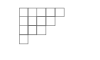
\includegraphics[scale=0.6]{../spherical-elastic/youngdiagram-ex.pdf}
	\end{center}
	
	\vspace{-0.8cm}
	
	Young diagrams  are said to be of some shape $\lambda:(\lambda_1,\lambda_2,...,\lambda_k)$, where $\lambda_i$ refers to the depth of row $i$ and $\lambda_{i+1}\leq\lambda_i\leq\lambda_{i-1}$. Above: $(5,4,3,1)$
\end{frame}
\begin{frame}{$GL$ Decomposition cont.}
	We can then form a set of Young tableaux from diagrams by filling in the boxes from a set of ordered indices $\lbrace x_1,x_2,...,x_k\rbrace$ corresponding to tensor components $T^{x_1x_2...x_k}$. 
	\begin{center}
		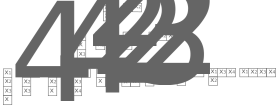
\includegraphics[scale=0.3]{../spherical-elastic/youngtableaux-ex.pdf}
	\end{center}
	A standard tableu is one filled with indices $x_i$ (without repeats) with entries increasing in index $i$ down each column and across (to the right) rows.
\end{frame}

\begin{frame}{$GL$ Decomposition cont.}
	Each of these standard tableaux correspond to an invariant subspace under $S_k$.
	
	\medskip
	
	These invariant subspaces may be constructed by correspond products of symmetrizers $s$ and antisymmetrizers $a$:
	$$
	s_{\lambda} = \prod_{\mathcal{I}\in \text{Cols}(\lambda)}\mathcal{S}(\mathcal{I})
	$$
	$$
	a_{\lambda} = \prod_{\mathcal{I}\in \text{Rows}(\lambda)}\mathcal{A}(\mathcal{I})
	$$
	\begin{center}
		where $\mathcal{S}$ and $\mathcal{A}$ act component-wise as:
	\end{center}
	$$
	\big[\mathcal{S}(\mathcal{I})T\big]_{ijk...}= \sum_{\sigma_{\mathcal{I}}}T_{\sigma_{\mathcal{I}}(ijk...)}
	$$
	$$
	\big[\mathcal{A}(\mathcal{I})T\big]_{ijk...}= \sum_{\sigma_{\mathcal{I}}}\text{sgn}(\sigma_{\mathcal{I}})T_{\sigma_{\mathcal{I}}(ijk...)}
	$$
\end{frame}

\begin{frame}{$O$ Decomposition}
	Orthogonal group $O$, preserves inner product between vectors $<\cdot , \cdot >$. defined by means of a metric tensor $g_{ij}$ , which transforms as a second rank tensor under some transformation $R$ as:
	$$
	g_{x_1x_2}\rightarrow g_{x'_1x_2'} = R_{x_1'}^{x_1} R_{x_2'}^{x_2}g_{x_1x_2}
	$$
	Contractions of arbitrary tensors $T$ with $g_{ij}$ are invariant under $O$.
	
	\medskip
	
	For example, consider the rank-3 covariant $T^{ijk}$:
	$$
	g_{i'j'}T^{i'j'k'} = S^{k'}= R_{i'}^{i} R_{j'}^{j} g_{ij}R_{i}^{i'} R_{j}^{j'}R_k^{k'}T^{ijk} = R_k^{k'} S^k
	$$
	so that $S$ acts like an invariant vector subspace under $O$.
\end{frame}
\begin{frame}{$SL$ Decomposition}
	Special linear group $SL$ of transformations is defined as invertible linear transformations with determinant equal to positive one.
	
	\medskip
	
	Under $SL$, orientation and volume are preserved, where volume is defined as the contraction of a tensor with the fully antisymmetric tensor $\epsilon_{ijk}$, which transforms under $R\in GL(3)$ as:
	$$
	\epsilon_{x_1x_2x_3} \rightarrow\epsilon_{x_1'x_2'x_3'} =\text{det}(R) R_{x_1'}^{x_1} R_{x_2'}^{x_2}R_{x_3'}^{x_3}\epsilon_{x_1x_2x_3} 
	$$
	Similar to the case of $g_{ij}$ in $O$, contractions with $\epsilon_{ijk}$ of arbitrary tensors yield $SL$ invariant subspaces.
\end{frame}

\begin{frame}{$SO(3)$ Decompositions}
	\small
	In $SO(3)$, we may use all of the above (Young, $g_{ij}$, $\epsilon_{ijk}$):
	
	\medskip
	
	$\bullet$ Young symmetrizers return a set of tensors of known symmetries (under index permutation).
	
	\medskip
	
	
	$\bullet$ Contractions with $g_{ij}$ along antisymmetric pairs of indices vanish.
	
	\medskip
	
	$\bullet$ Contractions with $\epsilon_{ij}$ along symmetric sets of indices vanish.
	
	\vspace{1cm}
	
	These may all be used together to decompose an arbitrary tensor into a set of symmetric, $SO(3)$ invariant, symmetric tensor subspaces. These then may be related to harmonic coefficients by way of the CG expansion from the $J_z$ basis given before.
\end{frame}
\begin{frame}{Example: Piezoelectric Tensors}
	
	The piezoelectric strain components $d_{ijk}$ are symmetric under $i,j$ so that:
	$$
	d_{ijk}=d_{jik}
	$$
	according to this symmetry, we see all Young tableaux but the following must disappear:
	\begin{center}
		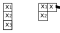
\includegraphics[scale=0.7]{../spherical-elastic/piezo_young.pdf}
	\end{center}defined component-wise (using the defining symmetry):
	\begin{align*}
		S_{ijk}&=\frac{1}{3}\big(d_{ijk}+d_{jki}+d_{ikj}\big)\\
		A_{ijk}&=\frac{1}{3}\big(2d_{ijk}-d_{jki}-d_{ikj}\big)\\
	\end{align*}
\end{frame}
\begin{frame}{Example: Piezoelectric Tensors}
	This may be derived as (adopting the convention of symmetrization before antisymmetrization):
	\begin{center}\small
		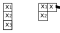
\includegraphics[scale=0.5]{../spherical-elastic/piezo_young.pdf}
		$$
		\mathcal{S}(ijk)\quad\quad \mathcal{A}(ij)\mathcal{S}(ik)
		$$
		\begin{align*}
			\mathcal{S}(ijk)d_{ijk}& =d_{ijk}+d_{ikj}+d_{kji}+d_{jki}+d_{kij}+d_{kji}\\
			&=2( d_{ijk}+d_{ikj}+d_{kji})\\
			\\
			\mathcal{A}(ik)\mathcal{S}(ij)d_{ijk}& =\mathcal{A}(ij)(d_{ijk}+d_{jik})\\
			&=d_{ijk}-d_{kji}+d_{jik}-d_{jki}\\
			&= 2d_{ijk}-d_{kji}-d_{jki}
		\end{align*}
	\end{center}
	Where the respective normalization coefficients (neglected here) may be derived from the diagram's shape via the hook-length formula.
\end{frame}
\begin{frame}{Example: Piezoelectric Tensors}
	\begin{center}
		Further decompose $A$ into the trace vector $v_i$:
		$$
		v^i =g_{jk}A^{ijk}
		$$
		
		and the traceless, symmetric tensor $b_{ij}$:
		$$
		b_{ij}=\frac{1}{2}\big(\epsilon_{i}^{mk}A_{mkj}+\epsilon_{j}^{mk}A_{mki}\big)
		$$
	\end{center}
\end{frame}

\begin{frame}{Group Representations}
	A representation $\rho_G$ of a group $G$ is a homomorphism from elements $g$ to a set of linear operators (square matrices). 
	
	\vspace{0.25cm}\small
	
	\begin{boxed2}
		
		\vspace{-.5cm}
		
		\textbf{Example: 3D Representation of $C_3$}
		
		Consider three identical points in 3D space forming an equilateral triangle.
		\begin{center}
			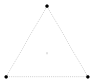
\includegraphics[scale=0.2]{../eqnn/c3triangle.pdf}
		\end{center}
		These clearly are symmetrical under three-fold rotations about the origin in the xy plane. These $C_3$ group actions act on this Cartesian basis with the representation $\rho$ defined:\tiny
		
		$$
		\rho(\mathbb{I}) = \begin{bmatrix}
			1&0&0\\
			0&1&0\\
			0&0&1\\
		\end{bmatrix}\quad 		\rho(C_3) = \begin{bmatrix}
			-\frac{1}{2}&-\frac{\sqrt{3}}{2}&0\\
			\frac{\sqrt{3}}{2}&-\frac{1}{2}&0\\
			0&0&1\\
		\end{bmatrix}\quad 
		\rho(C_3^2) = \begin{bmatrix}
			-\frac{1}{2}&\frac{\sqrt{3}}{2}&0\\
			-\frac{\sqrt{3}}{2}&-\frac{1}{2}&0\\
			0&0&1\\
		\end{bmatrix}
		$$
		
		\vspace{-0.5cm}
		
	\end{boxed2}
\end{frame}


\begin{frame}{Irreducible Representations (IRs)}
	For atomic arrangements, 3D group representations $\rho$ are  often reducible in terms of a direct sum of 'smaller' group representations $\rho^{(\alpha)}$:
	$$
	\rho = \bigoplus_{\alpha}c_{\alpha}\rho^{(\alpha)}
	$$
	
	Maschke's theorem guarantees that any given representation is always decomposable as a direct sum of irreducible representations. 
	
	\vspace{0.3cm}
	
	This set may always be taken to satisfy:
	
	\medskip
	
	$\bullet$ Unitarity
	
	\medskip
	
	$\bullet$ Orthogonality
	
	\medskip
	
	$\bullet$ $\sum_{\alpha} d_{\alpha}^2 = N $ where $d_{\alpha} $ is the dimension of IR $\alpha$ and $N$ is the order
	
\end{frame}

\begin{frame}{IRs (cont.)}
	
	\begin{boxed2}
		
		\vspace{-.57cm}
		
		\textbf{Example: IRs of $D_3$} The previously shown representation of $C_3$ elements is reducible into a two-dimensional subspace and a one-dimensional subspace of $D_3$. 
		
		\vspace{-.12cm}
		
		$$
		\rho(\mathbb{I}) =
		\rho^{(2)}(\mathbb{I})\oplus\rho^{(1)}(\mathbb{I})
		=
		\begin{bmatrix}
			1&0\\
			0&1\\
		\end{bmatrix}
		\oplus 
		\begin{bmatrix}
			1
		\end{bmatrix}
		$$
		$$
		\rho(C_3)
		=\rho^{(2)}(C_3)\oplus\rho^{(1)}(C_3)=
		\begin{bmatrix}
			-\frac{1}{2}&-\frac{\sqrt{3}}{2}\\
			\frac{\sqrt{3}}{2}&-\frac{1}{2}\\
		\end{bmatrix}
		\oplus
		\begin{bmatrix}
			1
		\end{bmatrix}
		$$
		$$
		\rho(C_3^2) 
		=
		\rho^{(2)}(C_3^2)\oplus\rho^{(1)}(C_3^2)
		= 
		\begin{bmatrix}
			-\frac{1}{2}&\frac{\sqrt{3}}{2}\\
			-\frac{\sqrt{3}}{2}&-\frac{1}{2}\\
		\end{bmatrix}
		\oplus
		\begin{bmatrix}
			1
		\end{bmatrix}
		$$
		
		\vspace{-.3cm}
		
	\end{boxed2}
\end{frame}


\begin{frame}{Orthogonality Theorems}
	IRs are orthogonal in the following ways:
	$$
	\frac{1}{N}\sum_{g}\chi^{(\alpha)*}(g)\chi^{(\beta)}(g) = \delta_{\alpha\beta}
	$$
	$$
	\sum_{\alpha}\chi^{(\alpha)*}(c_k)\chi^{(\alpha)}(c_h)= \frac{N}{N_k}\delta_{kh}
	$$
	where $N$ is the number of elements in $G$ and $N_k$ is the number of elements in equivalence class $k$.
	
	\medskip
	
	This allows us to decompose reducible representations by determining the coeffecients of expansion $c_{\alpha}$ as:
	
	$$
	c_{\alpha} = \frac{1}{N}\sum_{g}\chi^{(\alpha)*}(g)\chi(g)
	$$ 
\end{frame}

\begin{frame}{Orthogonality Theorems (cont.) }
	\small
	\begin{boxed2}
		
		\vspace{-.41cm}
		
		\textbf{Example: d-shell Splitting in Octohedral Coordinations} 
		
		Take the Hydrogen-like orbitals $\psi_{\ell m}$ as a basis for spherically symmetric states. The d-shell orbitals are the basis functions of the $\ell=2$ representations.
		
		\medskip
		
		%conventionally given as:
		%	$$
		%	\lbrace xy, xz, yz, 2z^2-x^2-y^2, x^2-y^2 \rbrace
		%	$$
		The octohedral complex's symmetry group is $O$, with it's character table and the $\Gamma^{\ell=2}$ representation:
		$$
		\begin{array}{c|c c c c c}
			O & 1\langle \mathbb{I}\rangle  & 8\langle C_3\rangle  & 3\langle C_2\rangle  & 6\langle C_2'\rangle & 6\langle C_4^3\rangle \\
			\hline 
			(d)\ \Gamma^{\ell=2} & 5 & -1 & 1 & 1 & -1 \\
			A_1 & 1 &  1&  1&  1&  1\\
			A_2 & 1&  1&  1&  -1&  -1\\
			E & 2 & -1 & 2 & 0 & 0 \\
			T_1 & 3 & 0 & -1 & -1 &1\\
			T_2 & 3 & 0 & -1 & 1 &-1\\
		\end{array}
		$$
		Orthogonality then gives $\gamma^{\ell=2}=E\oplus T_2$. In practice, this results in a 5-fold degeneracy being lifted into a two- and three-fold degeneracy.
		
		\vspace{-.3cm}
		
	\end{boxed2}
\end{frame}
\begin{frame}{Basis Functions}
	Every representation of a group inherits a vector space on which it has a natural action. This vector space is spanned by a chosen set of basis functions $\vert \psi^{\alpha}_i\rangle$.
	
	\vspace{0.5cm}
	
	\begin{itemize}
		\item 	An irrep $\Gamma^{\alpha}$'s components are determined by basis:
		$$\Big(\Gamma^{\alpha}(g)\Big)_{i}^{j}=\langle\psi^{\alpha}_j\vert \Gamma^{\alpha}(g) \vert \psi^{\alpha}_i\rangle$$
		
		\item Basis functions are said to ``transform as an irrep $\alpha$" if:
		$$
		\Gamma^{\alpha}(g) \vert \psi^{\alpha}_i\rangle =\sum_{j} \Big(\Gamma^{\alpha}(g)\Big)^j_i \vert \psi^{\alpha}_j\rangle
		$$
	\end{itemize}
	
	
\end{frame}


\begin{frame}{Basis Functions (cont.)}
	\small
	
	\begin{boxed2}
		
		\vspace{-.5cm}
		
		\textbf{Example: $3D$ Basis Functions of $D_3$}
		
		Consider previous $3D$ representation of $C_3$ rotations in $D_3$, which act on vectors $\vec{r}_{\rho}$:
		$$
		\vec{r}_{\rho}=\begin{bmatrix}
			x\\y\\z
		\end{bmatrix} = \vec{r}_{\rho^{(2)}}\oplus\vec{r}_{\rho^{(1)}} =\begin{bmatrix}
			x\\y
		\end{bmatrix}\oplus\begin{bmatrix}
			z
		\end{bmatrix}
		$$
		Clearly, $x,y$ is a basis transforming as $\Gamma^{2}$ and $z$ is a basis for $\Gamma^1$.
		
	\end{boxed2}
	
	\begin{boxed2}
		
		\vspace{-.41cm}
		
		\textbf{Example: Tight Binding} 
		
		The tight binding approximation often uses localized Hydrogen-like orbitals $\psi_{nm}^{\ell}$ as a basis for many-body systems
		
		\vspace{-.3cm}
		
	\end{boxed2}
	
\end{frame}

\begin{frame}{Projection Operators}
	If we have an explicit form for IR $\alpha$, we may project an arbitrary function onto the $k$-th basis function $f^{\alpha}_k$ of IR $\alpha$ with $\hat{P}_{\alpha}^{kk}$:
	$$
	\hat{P}_{\alpha}^{kk} = \frac{d_{\alpha}}{N}\sum_g \big[\Gamma^{kk}_{\alpha}(g) \big]^* O(g)
	$$
	where $d_{\alpha}$ is the dimensional of IR $\alpha$, and then we have:
	$$
	f_{\alpha}^k(\vec{r}) = \hat{P}_{\alpha}^{kk}f(\vec{r})
	$$
	From the characters alone, we may project a function onto it's total $\alpha$ subspace with $\hat{P}_{\alpha}$:
	$$
	\hat{P}_{\alpha} = \sum_k\hat{P}^{kk}_{\alpha} = \frac{d_{\alpha}}{N}\sum_{g}\chi^{(\alpha)*}(g)\hat{O}(g)
	$$
	
	
\end{frame}

\begin{frame}{Coupling Coefficients}
	Consider a direct product decomposition of some irreps $\Gamma$:
	$$
	\Gamma^{\alpha}\otimes\Gamma^{\beta}=\bigoplus_{\gamma}c_{\alpha\beta\gamma}\Gamma^{\gamma}
	$$
	
	Products of basis functions $u^{\alpha}_iv^{\beta}_j$ then decompose similarly into a direct sum of irreps with basis functions $\psi_{n}^{\gamma}$ via the coupling coefficients $U_{\alpha i \beta j}^{\gamma n}$ as:
	$$
	\psi_{n}^{\gamma}= \sum_{i,j}U_{\alpha i \beta j}^{\gamma n}u^{\alpha}_iv^{\beta}_j
	$$
	
	\begin{boxed2}\tiny
		
		\vspace{-.61cm}
		
		\textbf{Example: Clebsch-Gordan Coefficients} 
		
		The Clebsch-Gordan coefficients $C^{\ell_f  m_f}_{\ell_1  m_1\ell_2 m_2}$ are the coupling coefficients of $SO(3)$, which relate tensor product spaces of spherical harmonics $Y^{\ell}_m$ to direct sums of spherical harmonics.
		$$
		Y_{\ell_1}^{m_1}(\Omega)Y_{\ell_2}^{m_2}(\Omega)=\sum_{\ell_3, m_3}\sqrt{\frac{(2\ell_1+1)(2\ell_2+1)}{4\pi(2\ell_3+1)}}C^{\ell_3m_3}_{\ell_1m_1\ell_2m_2}C^{\ell_30}_{\ell_1 0\ell_2 0}Y_{\ell_3m_3}(\Omega)
		$$
		
		\vspace{-.3cm}
		
	\end{boxed2}
	
\end{frame}


\end{document}